\documentclass{beamer}
\usepackage{filecontents}



%construct dynamic page
\setbeamercovered{highly dynamic}
\newcounter{saveenumi}
\newcommand{\seti}{\setcounter{saveenumi}{\value{enumi}}}
\newcommand{\conti}{\setcounter{enumi}{\value{saveenumi}}}
\resetcounteronoverlays{saveenumi}

%set color and initial
\usetheme[progressbar=frametitle]{metropolis}
\definecolor{mygreen}{rgb}{.125,.5,.25}
\usecolortheme[named=mygreen]{structure}
\setbeamertemplate{frame numbering}[fraction]
\useoutertheme{metropolis}
\useinnertheme{metropolis}
\usefonttheme{metropolis}
\usecolortheme{spruce}
\setbeamercolor{background canvas}{bg=white}

\title{Ground Shaking Prediction}
\subtitle{with Graph Nueral Network}
\author{Phiphat Chomchit}
\institute{Chiang Mai University}

\begin{document}
	% Fill color in block
	\metroset{block=fill}
	
	\begin{frame}
		\titlepage
	\end{frame}
	
	\begin{frame}[t]{Basic Seismic Knowlendge}
		
		\begin{enumerate}
			\item \textbf{Earthquake} is the sudden fracture and movement of rocks inside the Earth. 
			Part of the energy released produces seismic waves, like P, S, and surface waves that 
			travel outward in all directions from the point of initial rupture.
			\item \textbf{Hypocenter} or Focus the point below the epicenter at which an earthquake
			begins.
			\item \textbf{Epicenter} the point (map location) on the Earth’s surface directly above 
			the hypocenter or focus of an earthquake.
			\seti
		\end{enumerate}
		
	\end{frame}
	
	\begin{frame}[t]{stick-slip model}
		\begin{figure}
			\centering
			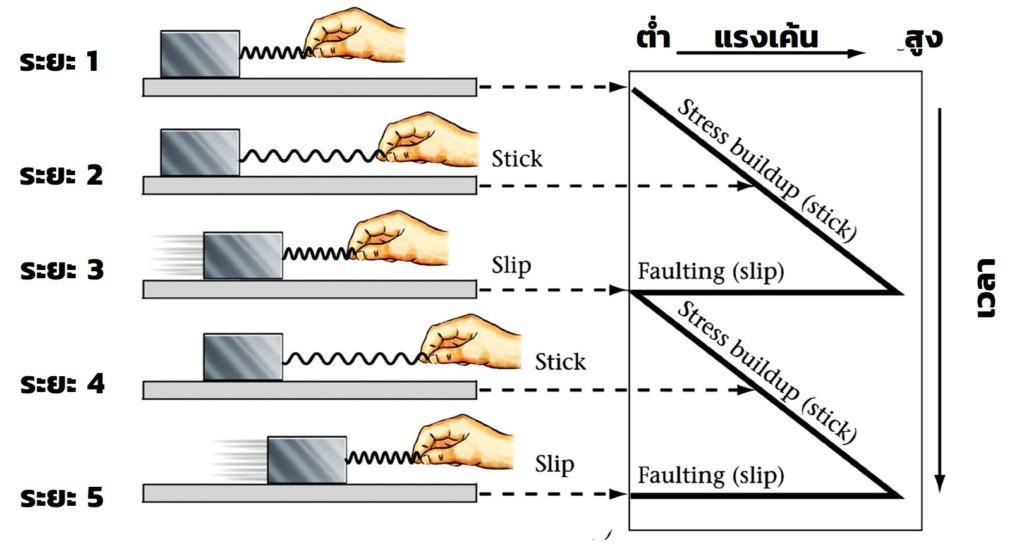
\includegraphics[scale=0.5]{stick.jpg}
			\caption{sick-slip model}
		\end{figure}
	\end{frame}
	
	\begin{frame}[t]{Basic Seismic Knowlendge}
		\begin{enumerate}
			\conti
			\item \textbf{P Wave} is the primary body wave; the first seismic wave detected by 
			seismographs; able to move through both liquid and solid rock. Also called compressional or 
			longitudinal waves, they compress and expand (oscillate) the ground back and forth in the 
			direction of travel, like sound waves that move back and forth as the waves travel from source 
			to receiver. P wave is the fastest wave.
			
			\item \textbf{S Waves} is shear waves that are secondary body waves that oscillate the ground 
			perpendicular to the direction of wave travel. They travel about 1.7 times slower than P waves. 
			Because liquids will not sustain shear stresses, S waves will not travel through liquids like water, 
			molten rock, or the Earth’s outer core. S waves produce vertical and horizontal motion in the 
			ground surface. 
			\seti
		\end{enumerate}
	\end{frame}
	
	\begin{frame}[t]{Body wave and surface wave}
		\begin{figure}
			\centering
			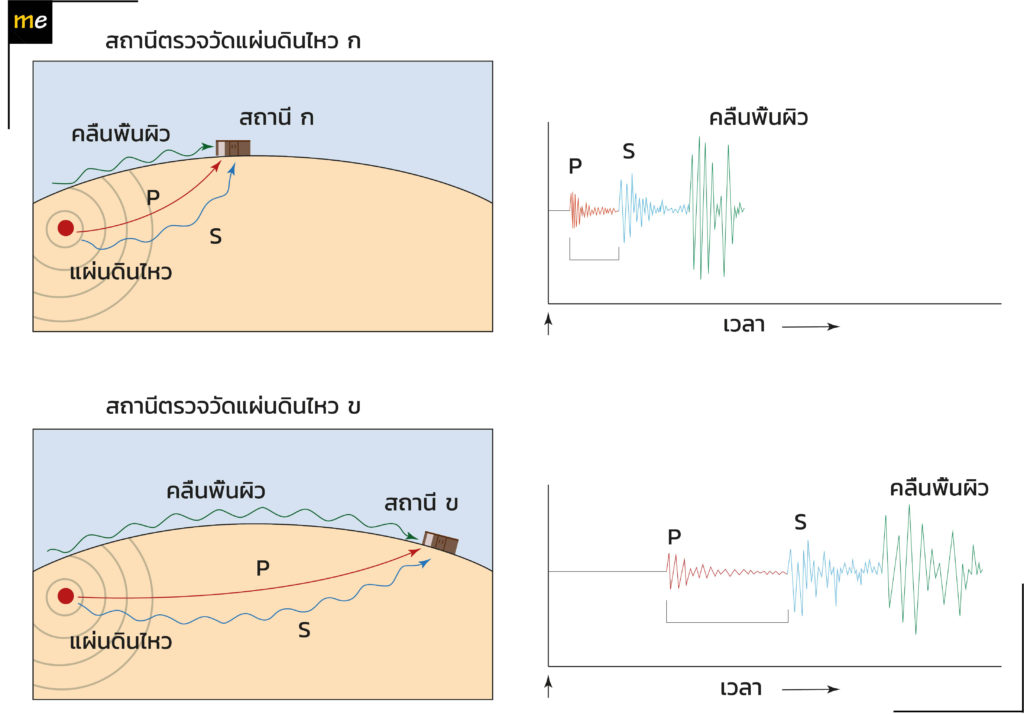
\includegraphics[scale=0.8]{station.jpg}
			\caption{P-wave, S-wave and surface wave}
		\end{figure}
	\end{frame}
	
	\begin{frame}[t]{Epicenter and Hypocenter}
		\begin{figure}
			\centering
			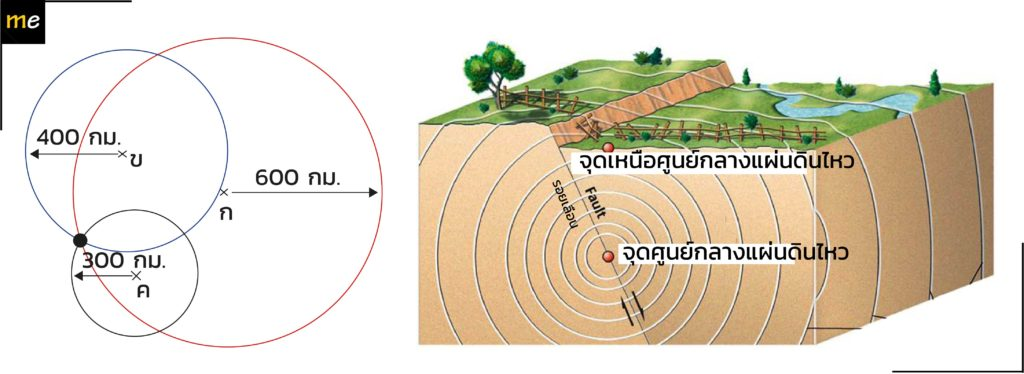
\includegraphics[scale=0.8]{velocity.jpg}
			\caption{Epicenter and Hypocenter}
		\end{figure}
		$V = \frac{S}{T}$
		
		$$T_p - T_s = \frac{S}{V_p} - \frac{S}{V_s}$$
	\end{frame}
	
	
	\begin{frame}[t]{Basic Seismic Knowlendge}
		\begin{enumerate}
			\conti
			\item \textbf{Peak Ground Acceleration} is a largest increase in velocity recorded by a particular station during 
			an earthquake. (Commonly called PGA) 
			\seti
		\end{enumerate}
		
		\begin{figure}
			\centering
			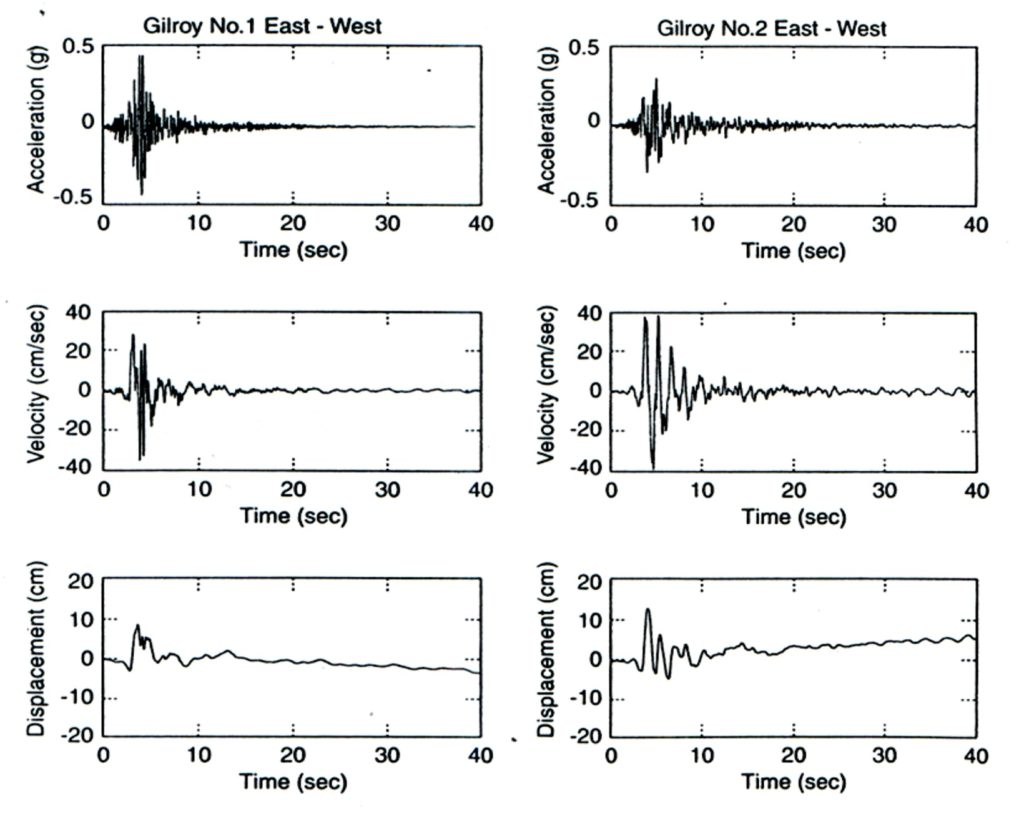
\includegraphics[scale=0.35]{pga.jpg}
			\caption{PGA, PGV, PGD}
		\end{figure}
	\end{frame}
	
	\begin{frame}[t]{Basic Seismic Knowledge}
		\begin{enumerate}
			\conti
			\item \textbf{Attenuation} is decrease in wave size, or amplitude, away from source. When you 
			throw a pebble in a pond, it makes waves on the surface that move out from the place where 
			the pebble entered the water. The waves are largest where they are formed and get smaller as 
			they move away.
			\seti
		\end{enumerate}
	
		\begin{figure}
			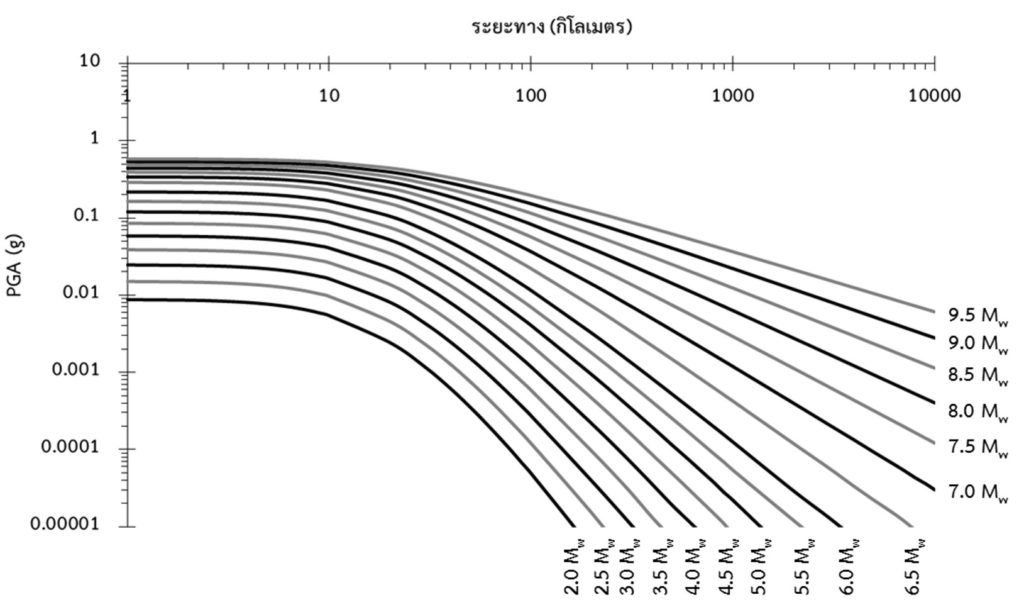
\includegraphics[scale=0.35]{anu.jpg}
			\caption{Attenuation}
		\end{figure}
	\end{frame}

	\begin{frame}[t]{Basic Seismic Knowledge}
		\begin{enumerate}
			\conti
			\item \textbf{Ground motion prediction model (GMPEs)}, also called ground-motion models 
			(GMMs) and attenuation relations, estimate the shaking (strong ground motion) that may occur 
			at a site if an earthquake of a certain magnitude occurs at a nearby location.
			\seti
		\end{enumerate}
		
		\begin{figure}
			\centering
			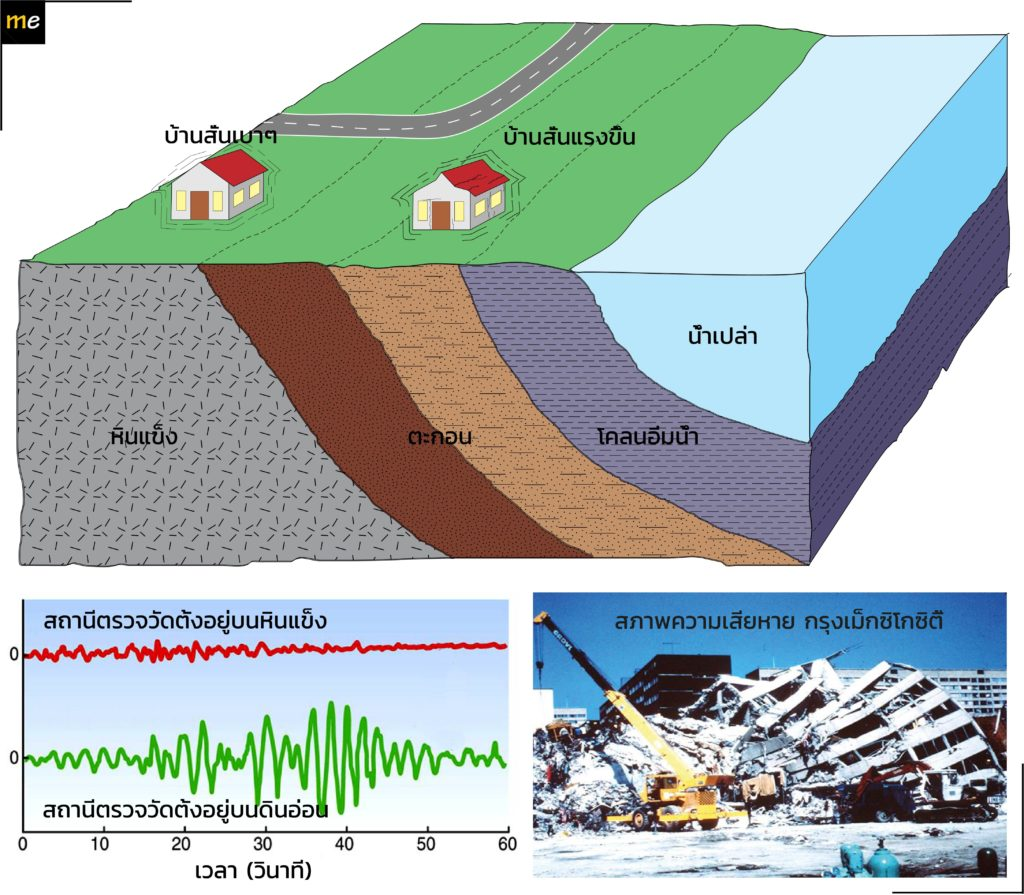
\includegraphics[scale=0.5]{shak.jpg}
			\caption{Ground Shaking}
		\end{figure}
	\end{frame}
	
	\begin{frame}[t]{Basic Seismic Knowlendge}
		\begin{enumerate}
			\conti
			\item \textbf{ShakeMap} The system is designed to combine instrumental measurements with information about local seismic site conditions and the earthquake source to estimate continuous shaking variations throughout a 
			spatial area. ShakeMap was implemented in other high-to-moderate-risk areas where rapid assessment of earthquakes is critical.
		\end{enumerate}
		\begin{figure}
			\centering
			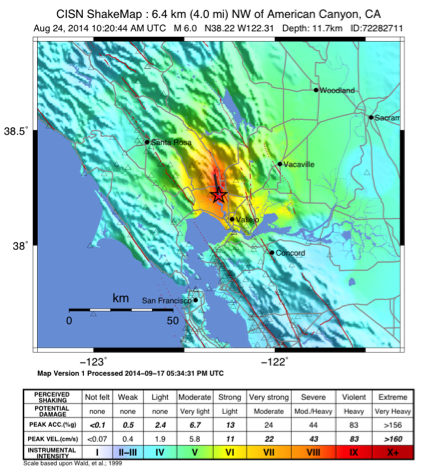
\includegraphics[scale=0.4]{example.png}
			\caption{Ground Shaking}
		\end{figure}
		
	\end{frame}

	\begin{frame}[t]{Review Papers}
		Why do we need machine learning?\\
		
		\vspace{10pt}
		\begin{enumerate}
			\item Parameters
			\begin{enumerate}
				\item Multilayer Perceptron
				\item Hybrid
				\item Genertic Programing
			\end{enumerate}
			\vspace{10pt}
			\item Waveform
			\begin{enumerate}
				\item Multilayer Perceptron
				\item Convolutional Neural Network
				\item Graph Neural Network
				\item Self Supervised Learning
			\end{enumerate}
		\end{enumerate}
	\end{frame}
	
	\begin{frame}[t]{Why do we need machine learning?}
		\begin{enumerate}
			\item Seismic data
				\begin{itemize}
					\item Imbalanced data
					\item Big data (Volume  Velocity and Variety )
				\end{itemize}
			\item Purpose of model
				\begin{itemize}
					\item rapid warning
					\item peak ground motion prediction
				\end{itemize}
		\end{enumerate}
	
		\begin{figure}
			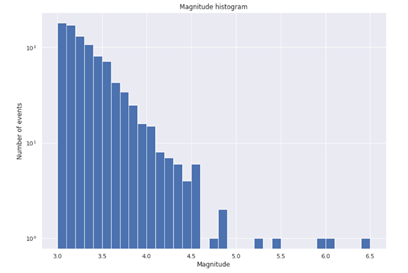
\includegraphics[scale=0.5]{imb.png}
			\caption{seismic data are long tail data.}
		\end{figure}
	\end{frame}

	\begin{frame}[t]{Multilayer Perceptron}
		\begin{figure}
			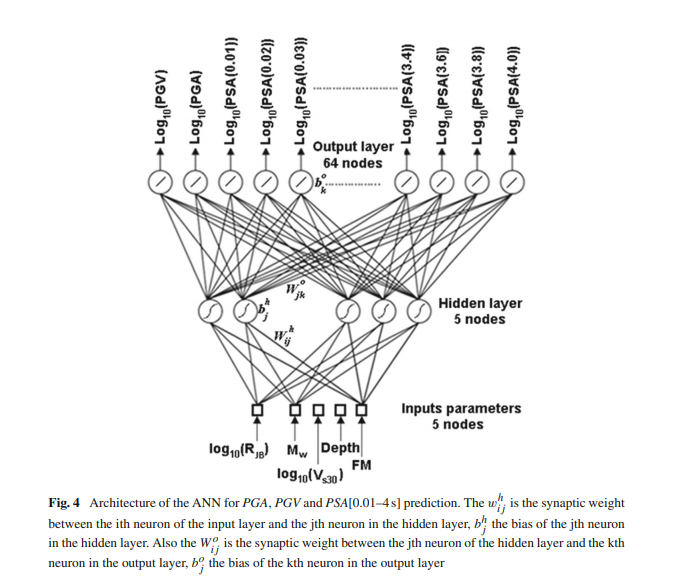
\includegraphics[scale=0.4]{mlp.png}
			\caption{PGA prediction with ANN}
		\end{figure}
		
	\end{frame}
	
	\begin{frame}[t]{Hybrid}
		\begin{figure}
			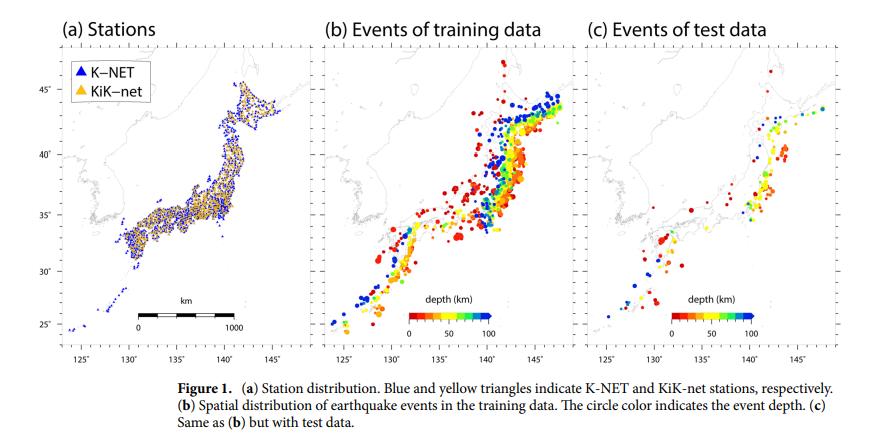
\includegraphics[scale=0.5]{hybrid.png}
			\caption{Hybrid model(GMPE + ERT)}
		\end{figure}
	\end{frame}
	
	
	\begin{frame}[t]{Convolutional Neural Network}
		\begin{figure}
			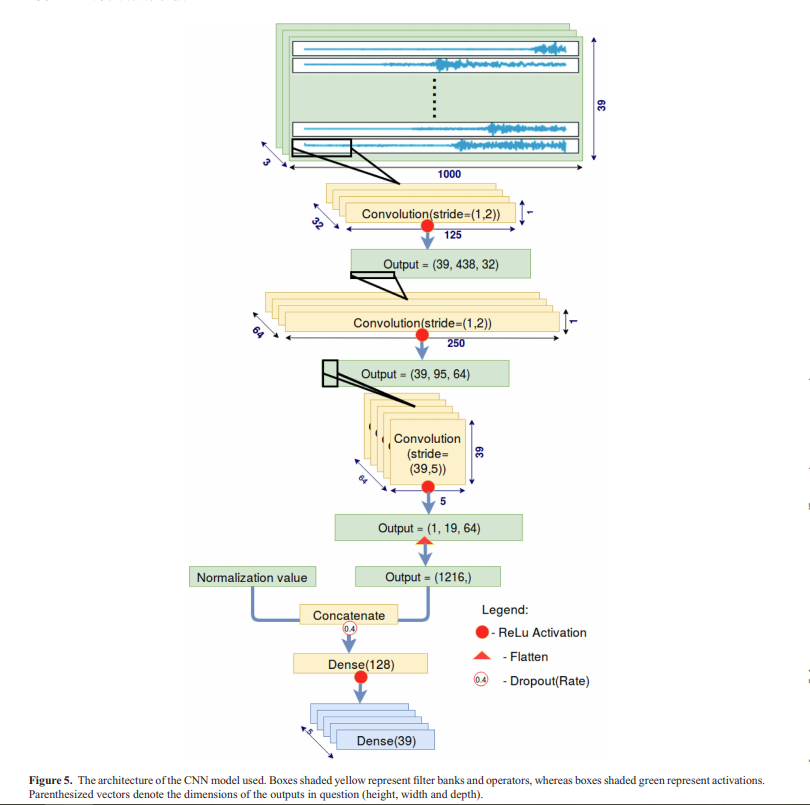
\includegraphics[scale=0.3]{cnn.png}
			\caption{CNN for rapid earthquake warning}
		\end{figure}
	\end{frame}
	

	
	\begin{frame}[t]{Graph Neural Network}
		\begin{figure}
			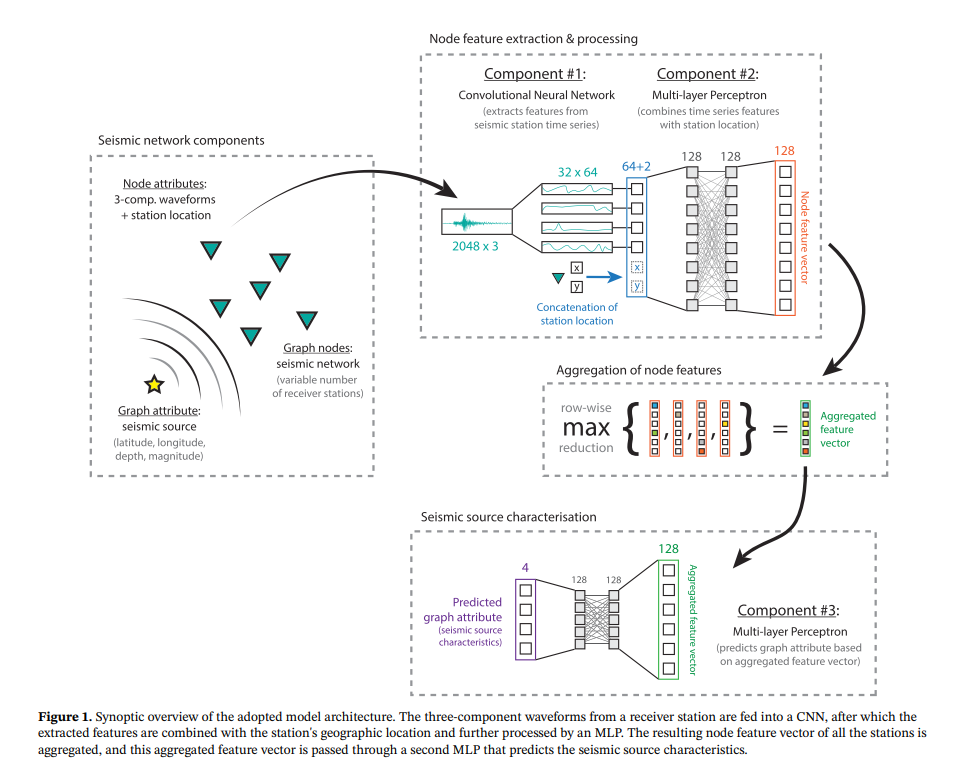
\includegraphics[scale=0.3]{gnn.png}
			\caption{Characterize source of earthquake with GNN}
		\end{figure}
	\end{frame}
	
	\begin{frame}[t]{Focus on my work}
		\begin{enumerate}
			\item Graph Neural Network
				\begin{itemize}
					\item spatial model
					\item temporal model
					\item static graph, dynamic signal
				\end{itemize}
			\item Semi-Supervised Learning and Self-Supervised Learning
				\begin{itemize}
					\item Unlabeled data
					\item Imbalanced data
				\end{itemize}
		\end{enumerate}
		
	\end{frame}
		\begin{frame}[t]{Focus on my work}
		\section{Graph Neural Network.}
		\begin{figure}
			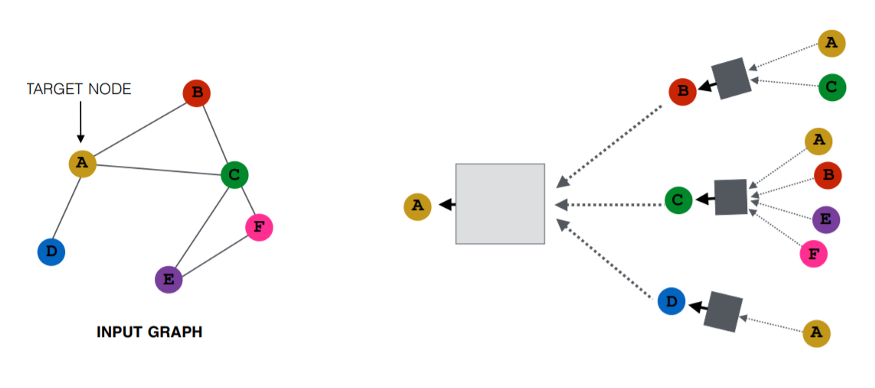
\includegraphics[scale=0.3]{node.png}
		\end{figure}
	\end{frame}

	\begin{frame}[t]{What is Graph Neural Network?}\vspace{10pt}
	
	\begin{block}{Graph definition}
		A graph $\mathcal{G}$ is defined as a tuple of a set of nodes/vertices $V$, and a set of edges /links $E$: $\mathcal{G}=(V,E)$. Each edge is a pair of two vertices, and represents a connection between them. 
	\end{block}
	For instance, let's look at the following graph:
	\begin{figure}
		\centering
		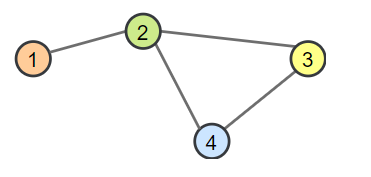
\includegraphics[scale=0.5]{sg.png}
		\caption{Example graph}
	\end{figure}
	
	The vertices are $V=\{1,2,3,4\}$,\\ and edges $E=\{(1,2), (2,3), (2,4), (3,4)\}$.
	\end{frame}

	\begin{frame}[t]{What is Graph Neural Network?}\vspace{4pt}
	\begin{block}{Definition of Adjacency Matrix}
		\vspace{0.5em}
		The \textbf{adjacency matrix} $A$ is a square matrix whose elements indicate whether pairs of vertices are adjacent, i.e. connected, or not. In the simplest case, $A_{ij}$ is 1 if there is a connection from node $i$ to $j$, and otherwise 0.
		\vspace{0.5em}
	\end{block}
	
	$$
	A = \begin{bmatrix}
		0 & 1 & 0 & 0\\
		1 & 0 & 1 & 1\\
		0 & 1 & 0 & 1\\
		0 & 1 & 1 & 0
	\end{bmatrix}
	$$
	
	keep in mind that $A$ is a symmetric matrix ($A_{ij}=A_{ji}$)
	\end{frame}

	\begin{frame}[t]{Graph Convolutions}\vspace{4pt}
	\begin{enumerate}
		\item GCNs are similar to convolutions in images in the sense that the "filter" parameters are typically shared over all locations in the graph. 
		\item At the same time, GCNs rely on message passing methods, which means that vertices exchange information with the neighbors, and send "messages" to each other.
	\end{enumerate}
	
	\begin{figure}
		\centering
		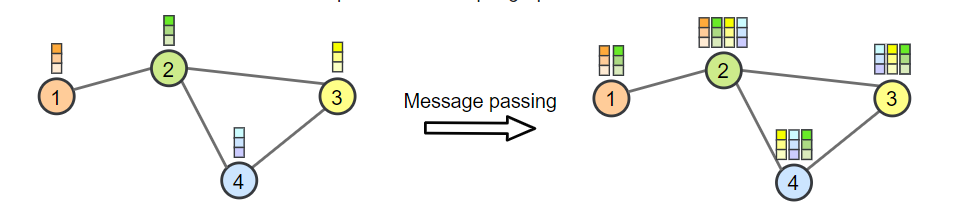
\includegraphics[scale=0.4]{sg2.png}
		\caption{Message passing between nodes}
	\end{figure}
	\end{frame}

	\begin{frame}[t]{Graph Convolutions}\vspace{4pt}
	Given the previous features of nodes $H^{(l)}$, the GCN layer is defined as follows:
	
	$$H^{(l+1)} = \sigma\left(\hat{D}^{-1/2}\hat{A}\hat{D}^{-1/2}H^{(l)}W^{(l)}\right)$$
	\begin{enumerate}
		\item $W^{(l)}$ is the weight parameters with which we transform the input features into messages ($H^{(l)}W^{(l)}$). 
		\item To the adjacency matrix $A$ we add the identity matrix so that each node sends its own message also to itself: $\hat{A}=A+I$. 
		\item $\hat{D}$ which is a diagonal matrix with $D_{ii}$ denoting the number of neighbors node $i$ has. 
		\item $\sigma$ represents an arbitrary activation function.
	\end{enumerate}
	\end{frame}

	\begin{frame}[t]{Example predict PM2.5 on graph station}
		\begin{figure}
			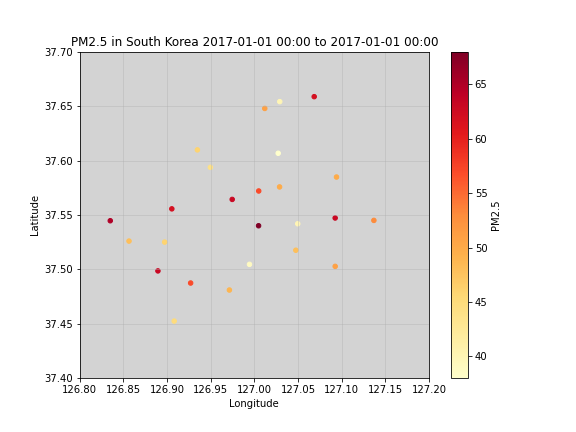
\includegraphics[scale=0.4]{station_pm.png}
			\caption{Predict PM2.5 with GNN}
		\end{figure}
	\end{frame}
	\begin{frame}[t]{Focus on my work}
		\section{Semi-Supervised Learning and Self-Supervised Learning.}
		
		\begin{figure}
			\centering
			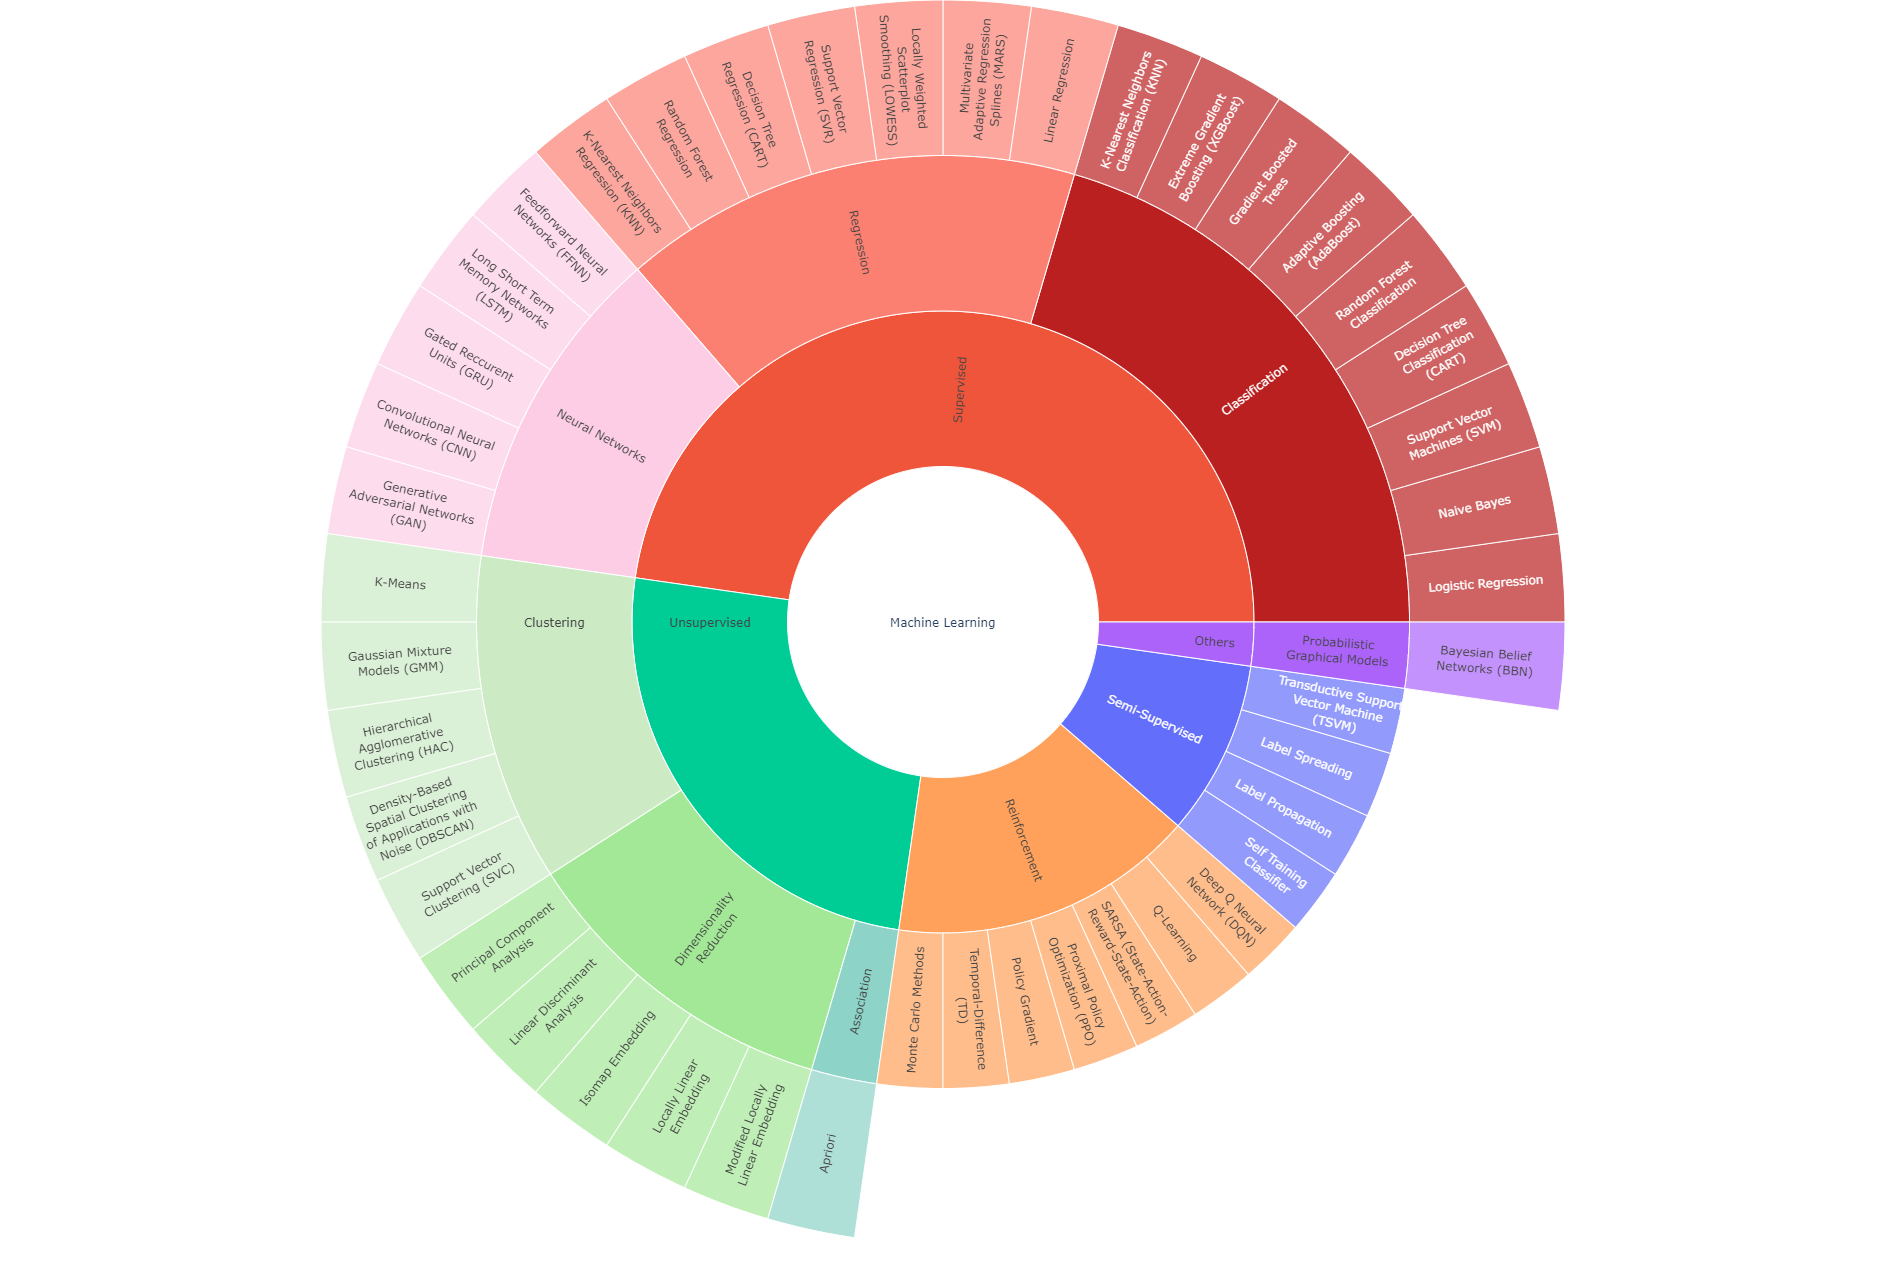
\includegraphics[scale=0.1]{newplot.png}
			\caption{Machine Learning}
		\end{figure}
	

	\end{frame}	

	\begin{frame}[t]{Self Supervised Learning?}\vspace{10pt}
		
		Contrastive self-supervised learning has outperformed supervised pretraining on many downstream tasks like segmentation and object detection.
		
		What if we can get labels for free for unlabelled data and train unsupervised dataset in a supervised manner? We can achieve this by framing a supervised learning task in a special form to predict only a subset of information using the rest. In this way, all the information needed, both inputs and labels, has been provided. This is known as self-supervised learning.
		
	\end{frame}
	
	\begin{frame}[t]{How it work?}\vspace{4pt}
		\begin{figure}
			\centering
			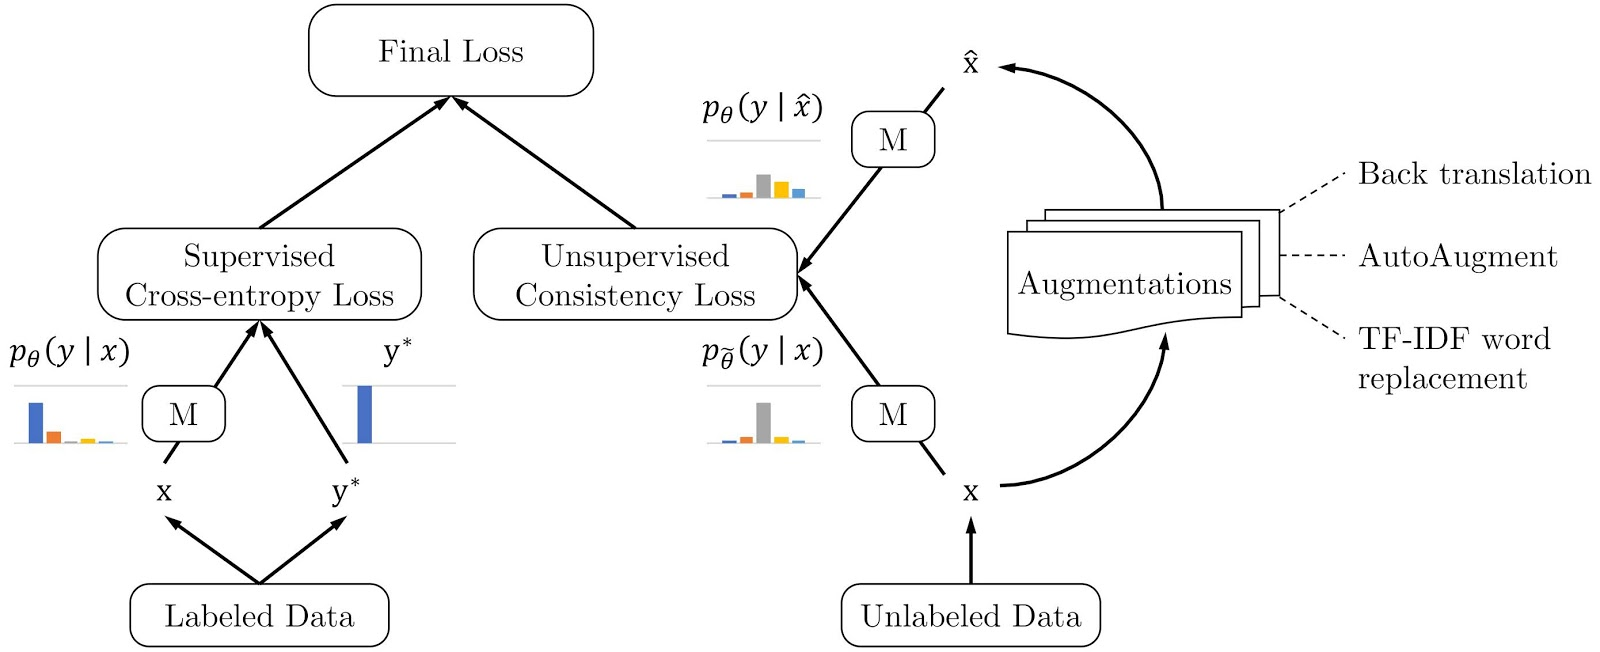
\includegraphics[scale=0.2]{google_semi.jpg}
			\caption{Semi and Self supervised learning}
		\end{figure}
	\end{frame}
	\begin{frame}[t]{Data Augmentation(Image data)}
		\begin{enumerate}
			\item Colorization
			\item Placing image patches in the right place
			\item Inpainting
		\end{enumerate}
	\end{frame}
	
	\begin{frame}{Colorization}\vspace{4pt}
		\begin{figure}
			\centering
			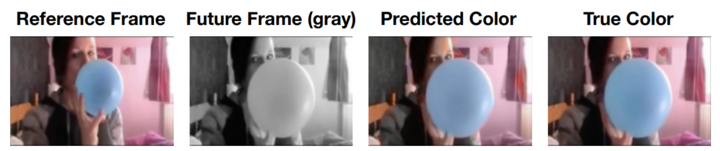
\includegraphics[scale=1]{color.png}
			\caption{change color tone}
		\end{figure}
	\end{frame}
	
	\begin{frame}{Placing image patches in the right place}\vspace{4pt}
		\begin{figure}
			\centering
			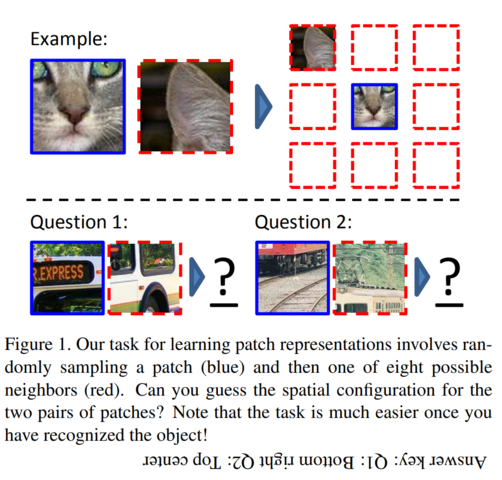
\includegraphics[scale=1]{placing.png}
			\caption{Location split image}
		\end{figure}
	\end{frame}
	
	\begin{frame}{Inpainting}\vspace{4pt}
		\begin{figure}
			\centering
			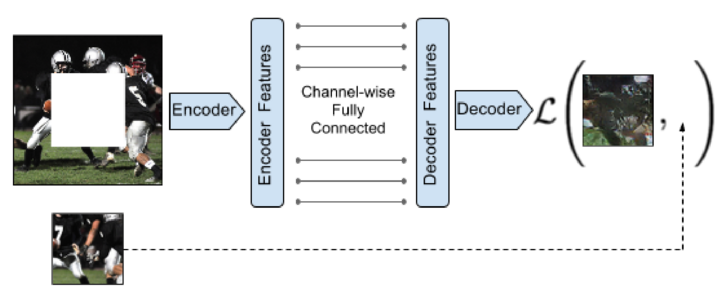
\includegraphics[scale=1]{inpainting.png}
			\caption{Autoencoder}
		\end{figure}
	\end{frame}
	
	
	\begin{frame}[t]{Fomulation}
		$$\mathcal{L}(\theta, \eta) = \mathbb{E}_{x, \mathcal{T}}\Big[\|\mathcal{F}_\theta(\mathcal{T}(x)) - \eta_x\|_2^2\Big]$$
		$$\underset{\theta, \eta}{\text{min }} \mathcal{L}(\theta, \eta)$$
		\begin{enumerate}
			\item $\mathcal{F}$ is a network parameterized by $\theta$.
			\item $\mathcal{T}$ is the augmentation.
			\item $x$ is an image.
			\item The expectation $\mathbb{E}[\cdot]$ is over the distribution
			of images and augmentations. For the ease of analysis, here
			we use the mean squared error $\|\cdot\|^2_2$
			\item $\eta_x$ is the representation of the image $x$
			
		\end{enumerate}
	\end{frame}
	
	\begin{frame}[t]{Clustering Image with Self-Supervised Learning (Birds)}
		\begin{figure}
			\centering
			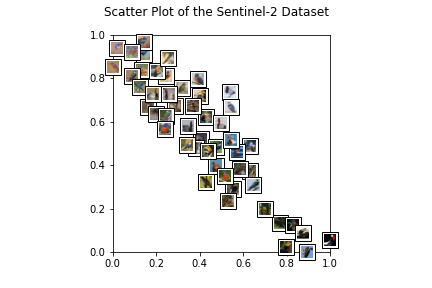
\includegraphics[scale=0.7]{birds.png}
			\caption{Embeding images on grid}
		\end{figure}
	\end{frame}

	\begin{frame}[t]{Clustering Earthquake Source with Self-Supervised Learning}
		\begin{figure}
			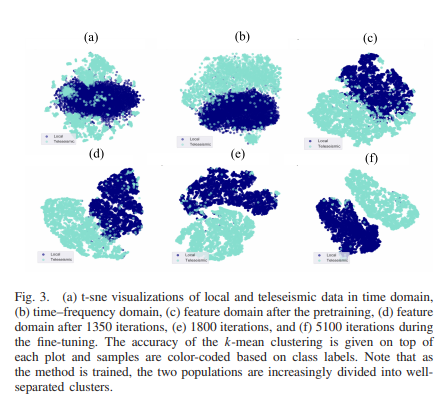
\includegraphics[scale=0.5]{self.png}
			\caption{self-supervised learning cluster local and teleseismic}
		\end{figure}
	\end{frame}

	\begin{frame}[t]{Why Graph and Self-Supervised?}
	\begin{enumerate}
		\item Resolve Imbalanced data problem
		\seti
	\end{enumerate}
	\begin{figure}
		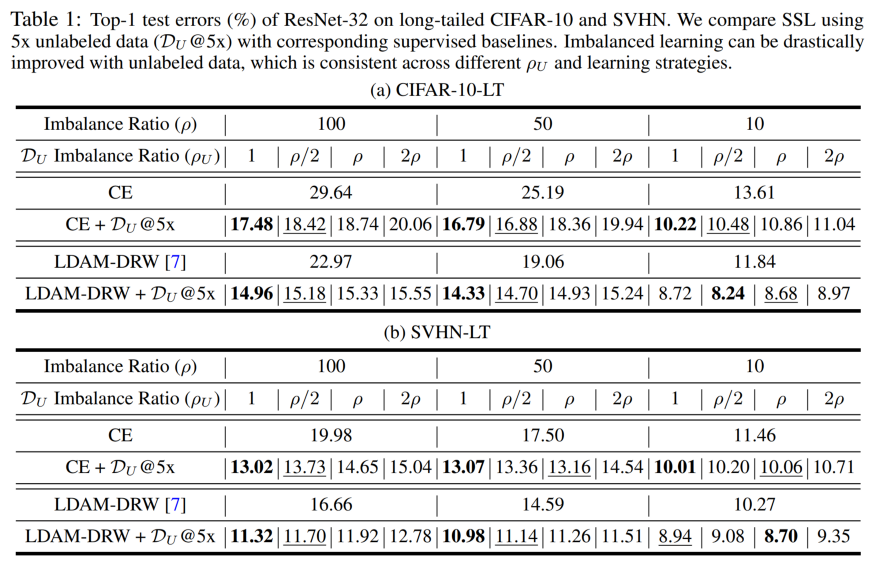
\includegraphics[scale=0.3]{result.png}
		\caption{SSL and imbalanced data}
	\end{figure}
	\end{frame}

	\begin{frame}[t]{Why Graph and Self-Supervised?}
		\begin{enumerate}
			\conti
			\item Represent Temporal and Spatial data
			\seti
		\end{enumerate}
	\begin{figure}
		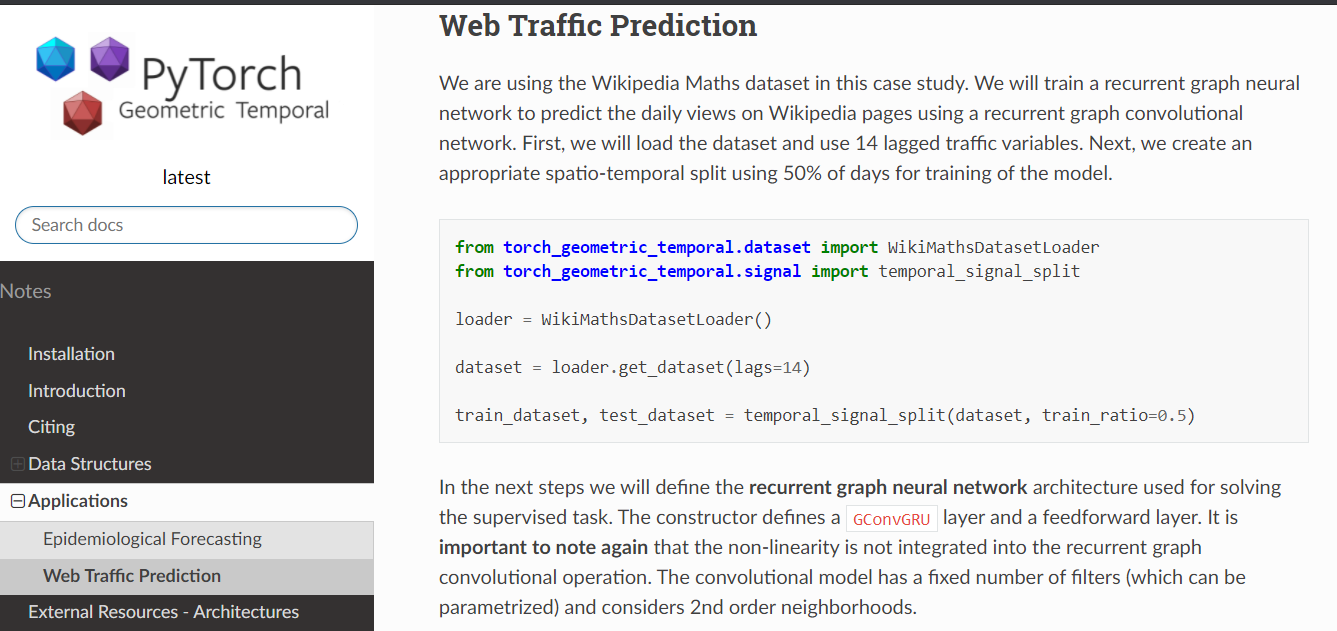
\includegraphics[scale=0.3]{web.png}
		\caption{web traffic prediction (GNN application example)}
	\end{figure}
	\end{frame}

	\begin{frame}[t]{Why Graph and Self-Supervised?}
		\begin{enumerate}
			\conti
			\item Self-supervised Training of Graph Convolutional Networks

		\end{enumerate}
		\begin{figure}
			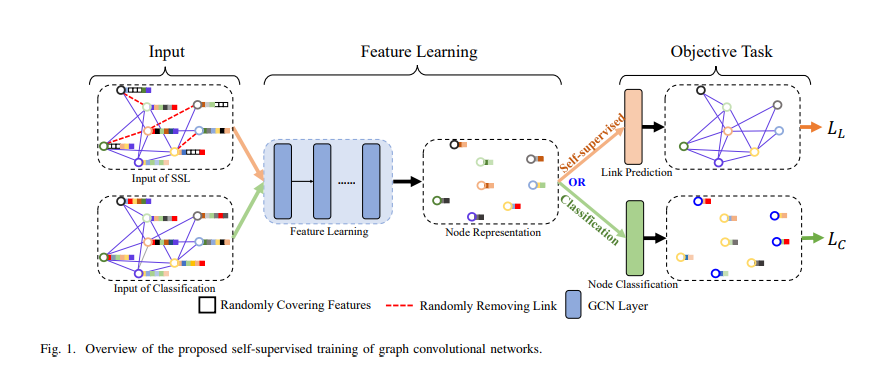
\includegraphics[scale=0.4]{self_graph.png}
			\caption{Self-supervised Training of Graph Convolutional Networks model }
		\end{figure}
	\end{frame}

	\begin{frame}[standout]
		Q/A
	\end{frame}
\end{document}